\documentclass{article}
\usepackage{graphics}
\usepackage{indentfirst}
\usepackage{amsmath}
\usepackage{algorithm}
\usepackage{algorithmic}
\usepackage{bm}
\usepackage{setspace}
\usepackage{graphicx}
\usepackage{float}
\author{Ruichen Wang}
\title{Variational Auto Encoder}
\begin{document}
\maketitle
\begin{abstract}
Variational auto-encoder \cite{DBLP:journals/corr/KingmaW13} is a very powful generative model. It can be used to generate or convert videos, images, texts, sounds etc. 
\end{abstract}

\tableofcontents
\section{What is VAE?} 
Variational auto-encoder is a brilliant combination of deep learning and variational inferece. It was proposed by Kingma in 2013. It provides a probabilistic manner for describing an observation in latent space. The encoder is aimed to describe a probability distribution for each latent attribute.
\begin{figure}[h]
\centering
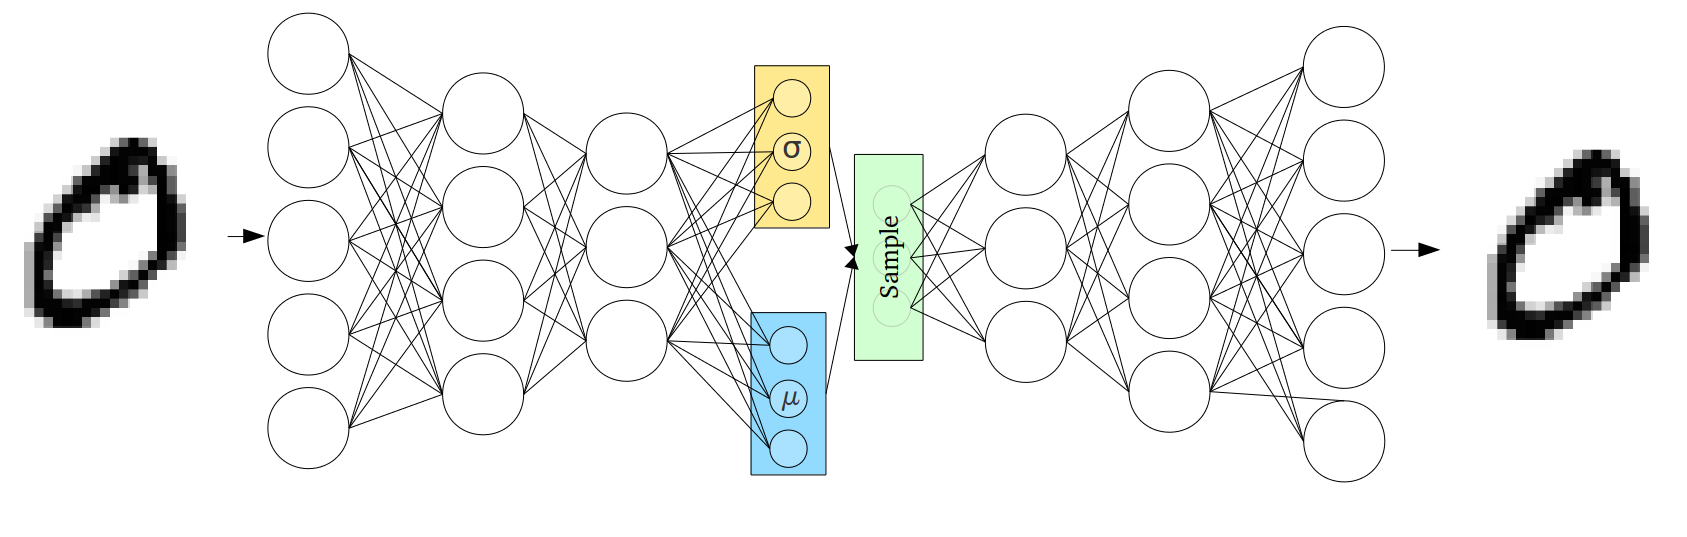
\includegraphics[width=5in,height=1.5in]{graph1}
\caption{VAE graph model}
\end{figure}
\subsection{Intuition}
In the past, we want the encoder to learn some  dimensions of input as the compressed feature. Using a variational autoencoder, we describe those latent dimensions in probabilistic terms.we'll now instead represent each latent attribute for a given input as a probability distribution. And we will perform random sampling on the distirbution to feed the decoder. We expecting the decoder can accurately reconstruct the input.

\subsection{Statisical motivation}
Suppose there exists some latent variable $z$ controls the observation $x$. We would like to infer the posterior $p_{\theta}(z|x)$
\begin{figure}[h]
\centering
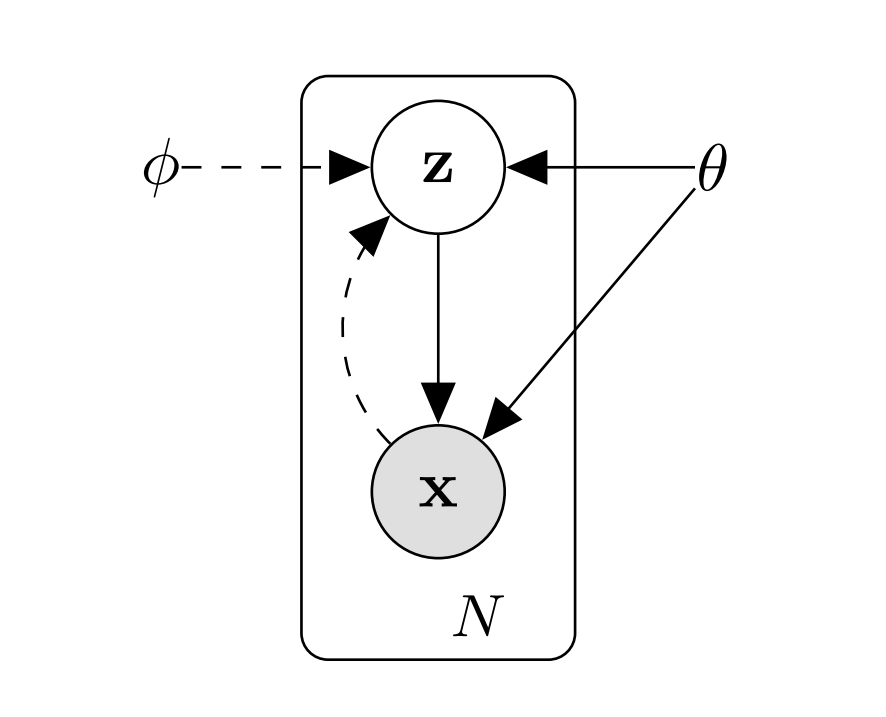
\includegraphics[width=2.5in,height=2in]{graph2}
\caption{Solid lines denotes the generative model $p_{\theta}(z)p_{\theta}(x|z)$. Dash lines denote the variational inference $q_{\phi}(z|x)$ which is a approximation of intractable $p_{\theta}(z|x)$.}
\end{figure}
$$p_{\theta}(z|x)=\frac{p_{\theta}(x|z)p_{\theta}(z)}{p_{\theta}(x)}=\frac{p_{\theta}(x|z)p_{\theta}(z)}{\int p_{\theta}(z)p_{\theta}(x|z)dz}$$

As we \textbf{do not} make the common simplifying assumptions about the marginal or posterior probabilities, the $\int p_{\theta}(z)p_{\theta}(x|z)dz$ is intractable, and EM algorithm or mean-field variational bayesian is also intractable.

So the VAE introduce a recognition model $q_{\phi}(z|x)$, which is a approximation to the posterior. Note the $\phi$ can not be computed from some closed-form expectation like mean-filed variational inference. It will be learned jointly with $\theta$.
\section{Method}
Remember the KL divergence can be used to measure the difference between distributions. We want to minimize the KL below:
$$min  D_{KL} (q_{\phi}(z|x)||p_{\theta}(z|x))$$
\subsection{Derivation of Variational Bound}
In this section, we will derivate the objective loss that VAE optimize.
\begin{align*}
D_{KL}(q_{\phi}(z|x)||p_{\theta}(z|x)) &= E_{q_{\phi}(z|x)} \left[ log \frac{q_{\phi}(z|x)}{p_{\theta}(z|x)} \right] \\
&= E_{q_{\phi}(z|x)}logq_{\phi}(z|x) -E_{q_{\phi}(z|x)} log p_{\theta}(z|x) \\
&= E_{q_{\phi}(z|x)}logq_{\phi}(z|x) -E_{q_{\phi}(z|x)}[log p_{\theta}(x,z)-log p_{\theta}(x)] \\
&= log p_{\theta}(x) + E_{q_{\phi}(z|x)}logq_{\phi}(z|x)- E_{q_{\phi}(z|x)}log p_{\theta}(x,z)
\end{align*}
As $log p_{\theta}(x)$ is fixed. The fomula can also be denoted as:
\begin{align*}
log p_{\theta}(x)=D_{KL}(q_{\phi}(z|x)||p_{\theta}(z|x)) + E_{q_{\phi}(z|x)}log p_{\theta}(x,z) -E_{q_{\phi}(z|x)}logq_{\phi}(z|x)
\end{align*}
Does this looks familiar to you? It is the evidence lower bound(ELBO). minimize the KL divergence is equal to maximize the ELBO. So now we convert our goal to :
\begin{align*}
max \mathcal{L} &= E_{q_{\phi}(z|x)}log p_{\theta}(x,z) -E_{q_{\phi}(z|x)}logq_{\phi}(z|x) \\
&= E_{q_{\phi}(z|x)}[logp_{\theta}(x|z)+logp_{\theta}(z)]-E_{q_{\phi}(z|x)}logq_{\phi}(z|x) \\
&= E_{q_{\phi}(z|x)}logp_{\theta}(x|z)-D_{KL}(q_{\phi}(z|x)||p_{\theta}(z))
\end{align*}
As you can see, the first term is the negative cross entropy $-H(q_{\phi}(z|x),p_{\theta}(x|z))$, which measures the reconstruction likelihood. The second term is regulation which encouraging the prior $p_{\theta}(z)$ to be closed to the aprroximate posterior $q_{\phi}(z|x)$.
\subsection{Reparameterization Trick}
To solve the problem, we invoked a distribution $q_{\phi}(z|x)$. As $z$ is sampled from some latent distirbution, it is not able to calculate the gradient. We use a method called \textbf{reparameterization trick} to rewrite the expectation in order to backpropagate.

\subsubsection{Example} 
Assume we have a normal distribution $q$ that is parameterized by $\theta$, specially $q_{\theta}(x)=N(\theta,1)$. We want to solve the below problem:
$$\mathop{\arg\min}_{\theta} E_{q}(x^{2})$$
It is quite obvious that $E(x^{2})=E(x)^{2}+D(x)=\theta^{2}+1$. $\theta=0$ is the answer. We want to see how reparameterization trick can help us solve this problem in calculating the gradients. 
\begin{align*}
\nabla_{\theta}E_{q}[x^{2}]&=\nabla_{\theta} \int q_{\theta}(x)x^{2}dx \\
&=  \int x^{2} \nabla_{\theta}q_{\theta}(x) \frac{q_{\theta}(x)}{q_{\theta}(x)} dx \\
&= \int q_{\theta}(x) x^{2} \nabla_{\theta} log q_{\theta}(x) dx \\
&= E_{q}[x^{2}\nabla_{\theta} logq_{\theta}(x)] \\
&= E_{q}[x^{2}(x-\theta)]
\end{align*}
As you can see the expectation is based on $q_{\theta}$. Using reparameterization trick can rewrite the expectation so that the distribution is independent with $\theta$. 

We make $p(\epsilon) \sim N (0,1)$, $x=\theta+\epsilon$. Hence: 
$$\nabla_{\theta}E_{q}[x^{2}]=E_{p}[\nabla_{\theta}(\theta+\epsilon)^{2}]=E_{p}(2(\theta+\epsilon))$$
Now we can also get our result $\theta=0$. Using reparameterization trick can also make the variance of gradience more stable.

\subsubsection{Reparametrization for the Posterior } 
First we sample a noise variable 
$$\epsilon \sim p(\epsilon)= N(0,1)$$
Then we apply a transform $g_{\phi}(\epsilon,x)$ that maps the random noise to a complex distribution. 
$$z=g_{\phi}(\epsilon,x)$$
Here we choose gaussian $z\sim q_{\mu,\sigma}(z)=N(\mu,\sigma)$, which is also can be denoted as :
$$z=g_{\mu,\sigma}(\epsilon)=\mu+\epsilon \cdot \sigma$$
The biggest advantage of this approach is that we many now write the gradient as:
$$\nabla_{\phi}E_{q(z|x)}[f(x,z)]=\nabla_{\phi}E_{p(\epsilon)}[f(x,g(\epsilon,x))]=E_{p(\epsilon)}[\nabla_{\phi}f(x,g(\epsilon,x))]$$
So we can write the frist term of ELBO as :
$$E_{q_{\phi}(z|x)}logp_{\theta}(x|z)=E_{p(\epsilon)}[logp_{\theta}(x|g(\epsilon,x))]=\frac{1}{L}\sum_{l=1}^{L}logp_{\theta}(x|g(\epsilon^{l},x)) $$
Now we take the sampling operation outside the network, which is sampling $\epsilon$ instead of $z$.
\begin{figure}[h]
\centering
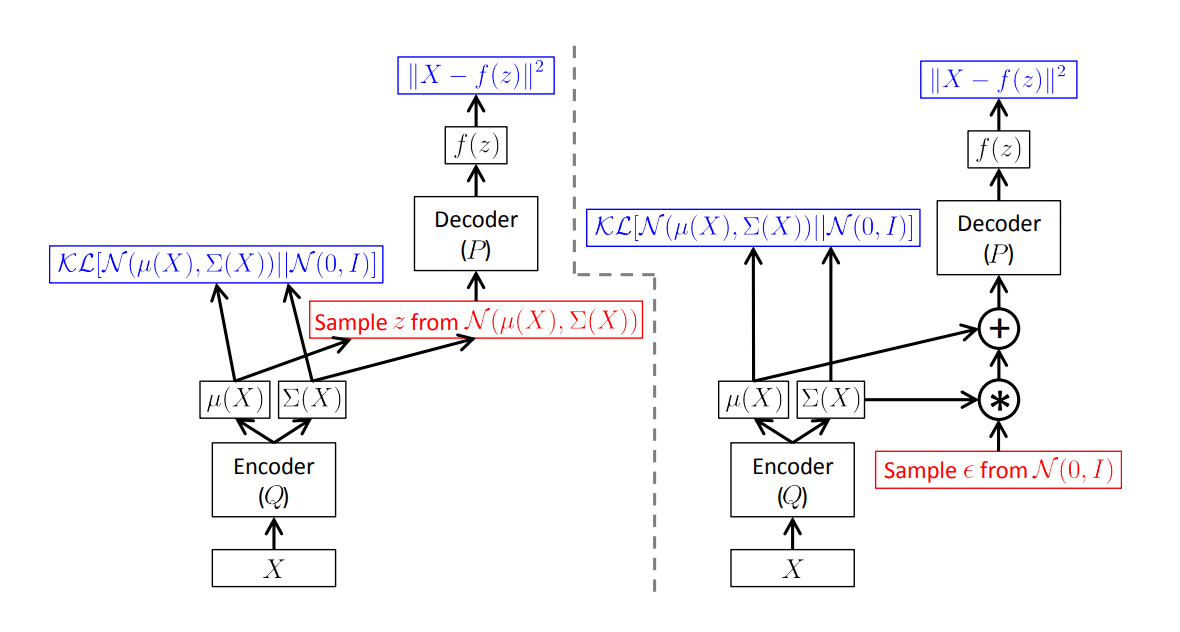
\includegraphics[width=5in,height=2.5in]{graph3}
\caption{Left without reparameterization trick. Right with it. The sampling operation is equivalent. But backpropagation can only be applied
to the right.\cite{DBLP:journals/corr/Doersch16}}
\end{figure}


\begin{figure}[h]
\centering
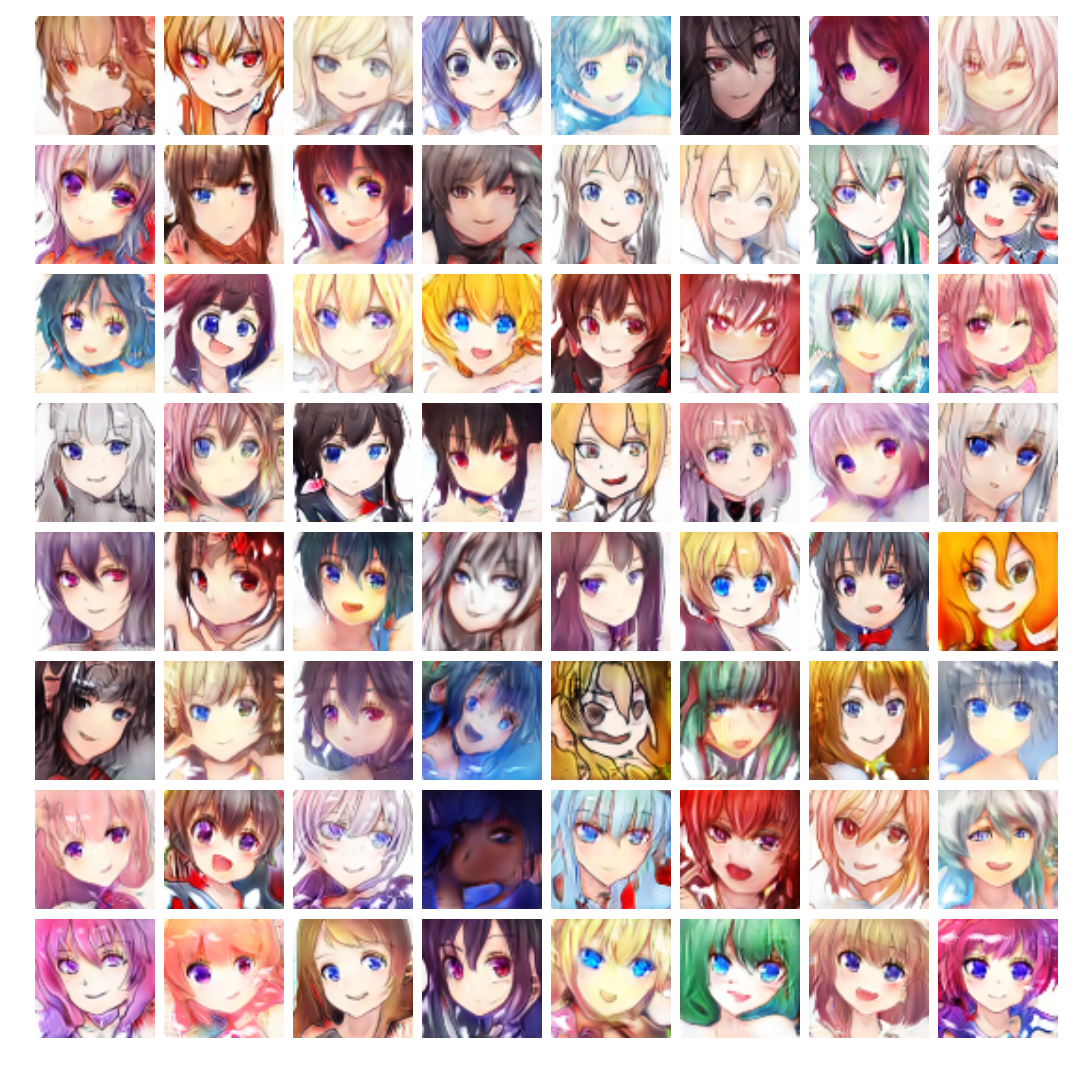
\includegraphics[width=5in,height=5in]{result1}
\caption{Generated images}
\end{figure}


\bibliographystyle{plain}
\bibliography{ref}

\end{document}


























